% Options for packages loaded elsewhere
\PassOptionsToPackage{unicode}{hyperref}
\PassOptionsToPackage{hyphens}{url}
%
\documentclass[
]{article}
\title{introduction}
\author{}
\date{\vspace{-2.5em}}

\usepackage{amsmath,amssymb}
\usepackage{lmodern}
\usepackage{iftex}
\ifPDFTeX
  \usepackage[T1]{fontenc}
  \usepackage[utf8]{inputenc}
  \usepackage{textcomp} % provide euro and other symbols
\else % if luatex or xetex
  \usepackage{unicode-math}
  \defaultfontfeatures{Scale=MatchLowercase}
  \defaultfontfeatures[\rmfamily]{Ligatures=TeX,Scale=1}
\fi
% Use upquote if available, for straight quotes in verbatim environments
\IfFileExists{upquote.sty}{\usepackage{upquote}}{}
\IfFileExists{microtype.sty}{% use microtype if available
  \usepackage[]{microtype}
  \UseMicrotypeSet[protrusion]{basicmath} % disable protrusion for tt fonts
}{}
\makeatletter
\@ifundefined{KOMAClassName}{% if non-KOMA class
  \IfFileExists{parskip.sty}{%
    \usepackage{parskip}
  }{% else
    \setlength{\parindent}{0pt}
    \setlength{\parskip}{6pt plus 2pt minus 1pt}}
}{% if KOMA class
  \KOMAoptions{parskip=half}}
\makeatother
\usepackage{xcolor}
\IfFileExists{xurl.sty}{\usepackage{xurl}}{} % add URL line breaks if available
\IfFileExists{bookmark.sty}{\usepackage{bookmark}}{\usepackage{hyperref}}
\hypersetup{
  pdftitle={introduction},
  hidelinks,
  pdfcreator={LaTeX via pandoc}}
\urlstyle{same} % disable monospaced font for URLs
\usepackage[margin=1in]{geometry}
\usepackage{graphicx}
\makeatletter
\def\maxwidth{\ifdim\Gin@nat@width>\linewidth\linewidth\else\Gin@nat@width\fi}
\def\maxheight{\ifdim\Gin@nat@height>\textheight\textheight\else\Gin@nat@height\fi}
\makeatother
% Scale images if necessary, so that they will not overflow the page
% margins by default, and it is still possible to overwrite the defaults
% using explicit options in \includegraphics[width, height, ...]{}
\setkeys{Gin}{width=\maxwidth,height=\maxheight,keepaspectratio}
% Set default figure placement to htbp
\makeatletter
\def\fps@figure{htbp}
\makeatother
\setlength{\emergencystretch}{3em} % prevent overfull lines
\providecommand{\tightlist}{%
  \setlength{\itemsep}{0pt}\setlength{\parskip}{0pt}}
\setcounter{secnumdepth}{-\maxdimen} % remove section numbering
\ifLuaTeX
  \usepackage{selnolig}  % disable illegal ligatures
\fi

\begin{document}
\maketitle

\hypertarget{introduction-to-the-lab}{%
\subsubsection{Introduction to the lab}\label{introduction-to-the-lab}}

4차 산업 시대에서 데이터를 분석하여 의미 있는 시사점을 찾아내는 것의
중요성은 점차 확대되고 있다. 호스피탈리티 산업이 서비스 중심임에도
불구하고 해당 산업과 관련된 많은 통계 및 자료들이 축적되고 있는 상황에서
데이터를 수집, 정리, 요약, 분석, 전략제시 등을 하는 것은 호스피탈리티
분야에서도 필요하며 빅데이터는 자료수집능력과 수집된 양이 크게 성장하여
기존 자료를 보관 및 분석하는 것에 큰 의미를 가지고 있다. 4차산업 융복합
연구소는 4차 산업 시대에서 빅데이터 활용은 호스피탈리티 분야에서
중요하게 여겨짐에 따라 데이터 수집, 분석, 전략제시 등 데이터 활용 목적의
기초 공부를 하고 있는 연구소이다.

\begin{center}\rule{0.5\linewidth}{0.5pt}\end{center}

\hypertarget{uxc5f0uxad6cuxc6d0-uxc18cuxac1c}{%
\subsection{연구원 소개}\label{uxc5f0uxad6cuxc6d0-uxc18cuxac1c}}

\hypertarget{uxae40uxcca0uxbbfc}{%
\subsubsection{김철민}\label{uxae40uxcca0uxbbfc}}

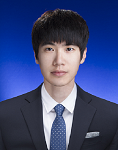
\includegraphics{images/figure2.png}

\begin{itemize}
\tightlist
\item
  학력사항 : 배재대학교 관광축제한류대학원 관광·호텔경영학과
  관광·호텔경영학 석사 재학 / 2021.03.\textasciitilde{} 배재대학교
  인문사회대학 공무원법학과(법학사) / 복수: 글로벌관광호텔학(경영학사) /
  2021.02. 卒
\item
  경력사항(일반경력): 한국커피칵테일교육원(KCCS) 광주센터 바텐더
  보조강사 근무 / 2019.07\textasciitilde2020.02 태국/필리핀/사이판 등
  현지 스쿠버다이빙 강사 및 가이드 근무 / 2016.04\textasciitilde2018.02
\item
  경력사항(군 경력): 대한민국 해병대 부사관(334기/중사 전역) / 대대 및
  단 본부 인사참모실 인사/행정 및 예산/회계 업무(3년)
\item
  경력사항(수상 경력):BARCHEF Global Competition 2019(바텐더 대회)
  장려상(클래식 부문) 수상
\item
  자격사항:중국어 사법통역사, 스쿠버다빙 강사, 응급처치 및
  AED(자동제세동기) 강사, 조주기능사, Jr.~Barchef(국제바텐더 Lv1) 등
\end{itemize}

-글상자-

\hypertarget{uxc1a1uxd615uxc6a9}{%
\subsubsection{송형용}\label{uxc1a1uxd615uxc6a9}}

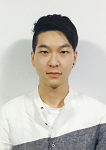
\includegraphics{images/figure3.png}

\begin{itemize}
\tightlist
\item
  학력사항 : 배재대학교 글로벌관광호텔학과, 상담심리학과(복수전공),
  호스피탈리티 융합(복수전공)
\item
  경력사항(일반경력):
\item
  경력사항(수상 경력):
\item
  자격사항: 워드프로세서 3급
\end{itemize}

-글상자-

\hypertarget{uxc774uxd638uxc81c}{%
\subsubsection{이호제}\label{uxc774uxd638uxc81c}}

보기:

\begin{itemize}
\tightlist
\item
  학력사항 : 배재대학교 호텔레저경영학과 재학,
  호스피탈리티SW융합(복수전공)
\item
  경력사항(일반경력):
\item
  경력사항(수상 경력):
\item
  자격사항:
\end{itemize}

-글상자-

\hypertarget{uxae40uxb3d9uxd604}{%
\subsubsection{김동현}\label{uxae40uxb3d9uxd604}}

보기:

\begin{itemize}
\tightlist
\item
  학력사항 : 배재대학교 호텔레저경영학과 재학,
  호스피탈리티SW융합(복수전공)
\item
  경력사항(일반경력):
\item
  경력사항(군 경력): 대한민국 보병 73사단 206연대 1대대 본부중대
  편성보급병 (병장 만기전역)
\item
  경력사항(수상 경력):
\item
  자격사항: 1종 운전면허 자격증, 태권도 3단 자격증 보유
\end{itemize}

-자기소개-

최근 AISW에 관심이 생겨 배우고 있는 연구원입니다. R과 R-STUDIO를
활용해서 데이터를 분석하는 작업을 배우고 있으며, 텍스트마이닝,
구글트렌드를 이용한 회귀분석, Python과 google colab을 활용하는 것을
배우고 있습니다. 개인 연구로는 관심분야인 텍스트마이닝을 활용하는 것을
진행하고 있습니다.

\hypertarget{uxae40uxc9c0uxc601}{%
\subsubsection{김지영}\label{uxae40uxc9c0uxc601}}

보기:

\begin{itemize}
\tightlist
\item
  학력사항 : 배재대학교 호텔레저경영학과 재학,
  호스피탈리티SW융합(복수전공)
\item
  경력사항(일반경력):
\item
  경력사항(수상 경력):
\item
  자격사항:워드프로세서 3급
\end{itemize}

-글상자-

\hypertarget{uxd55cuxc218uxc815}{%
\subsubsection{한수정}\label{uxd55cuxc218uxc815}}

\begin{itemize}
\tightlist
\item
  학력사항 : 배재대학교 호텔항공경영학과, 호스피탈리티SW융합(복수전공)
\item
  경력사항(일반경력):
\item
  경력사항(수상 경력):
\item
  자격사항: SMAT(서비스경영자격) 2급, MOS Power point, MOS Excel, MOS
  Word
\end{itemize}

-글상자-

\end{document}
